%! Author = Len Washington III
%! Date = 8/21/2023

% Preamble
\documentclass[chapter=7,section=1]{math252homework}

% Document
\begin{document}

In Problems 1--18 use Definition 7.1.1 to find $\laplace \{ f(t) \}$.
\begin{problems}
	\problem \[ f(t) = \left\{ \begin{array}{rr}
		-1, & 0 \leq t < 1\\
		1,	& t \geq 1
	\end{array} \right. \] % TODO: Problem 1
	\setcounter{problemsi}{3}
	\problem \[ f(t) = \left\{ \begin{array}{rr}
		2t+1, & 0 \leq t < 1\\
		0, & t \geq 1
	\end{array} \right. \] % TODO: Problem 4
	\setcounter{problemsi}{6}
	\problem~\begin{figure}[H]
				 \centering
				 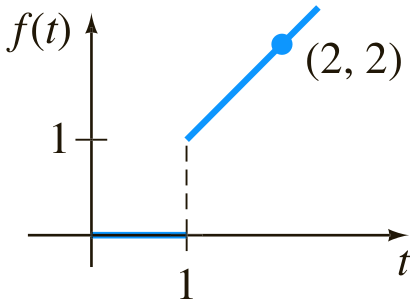
\includegraphics[width=0.4\textwidth]{7.7}
				 \caption{Graph for Problem \hyperref[prb:7]{\arabic{problemsi}}}
				 \label{fig:7}
	\end{figure} % TODO: Problem 7
	\setcounter{problemsi}{9}
	\problem~\begin{figure}[H]
				 \centering
				 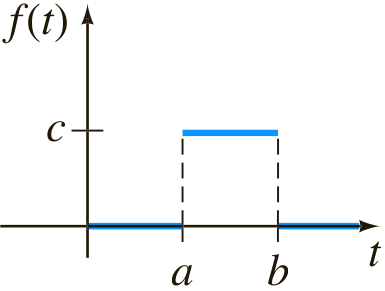
\includegraphics[width=0.4\textwidth]{7.10}
				 \caption{Graph for Problem \hyperref[prb:10]{\arabic{problemsi}}}
				 \label{fig:10}
	\end{figure} % TODO: Problem 10
\end{problems}

In Problems 19--37 use Theorem 7.1.1 to find $\laplace \{ f(t) \}$.
\begin{problems}[start=19]
	\problem \[ f(t) = 2t^{4} \] % TODO: Problem 19
	\setcounter{problemsi}{22}
	\problem \[ f(t) = t^{2} + 6t - 3 \] % TODO: Problem 23
	\problem \[ f(t) = -4t^{2} + 16t + 9 \] % TODO: Problem 24
	\problem \[ f(t) = (t+1)^{3} \] % TODO: Problem 25
	\setcounter{problemsi}{29}
	\problem \[ f(t) = (e^{t}-e^{-t})^{2} \] % TODO: Problem 30
	\problem \[ f(t) = 4t^{2} - 5\sin(3t) \] % TODO: Problem 31
	\setcounter{problemsi}{32}
	\problem \[ f(t) = \sinh(kt) \] % TODO: Problem 33
	\setcounter{problemsi}{34}
	\problem \[ f(t) = e^{t}\sinh(t) \] % TODO: Problem 35
\end{problems}

\end{document}